\documentclass[12pt,a4paper]{report}

\usepackage[utf8]{inputenc}
\usepackage[T1]{fontenc}
\usepackage[spanish]{babel}
\usepackage{tikz}
\usetikzlibrary{positioning,arrows.meta}
\usepackage{graphicx}
\usepackage{float}
\usepackage{geometry}
\usepackage{setspace}
\usepackage{amsmath}
\usepackage{amssymb}
\usepackage{hyperref}
\usepackage{listings}
\usepackage{xcolor}

\geometry{
left=3cm,
right=2.5cm,
top=3cm,
bottom=3cm
}

\setstretch{1.3}

\title{Simulación de Tormenta mediante Billboards y Sistemas de Partículas utilizando OpenGL}

\author{Diego Raúl Rivas Huanca \\
Alvarez Astete Jheeremy Manuel}

\date{\today}

\begin{document}

\maketitle

\tableofcontents

\clearpage

\chapter{Introducción}

La representación de fenómenos atmosféricos en tiempo real constituye uno de los problemas clásicos dentro del área de gráficos por computadora. Efectos como la lluvia, la nieve, la niebla o el humo pueden involucrar miles de elementos visibles de manera simultánea, lo que representa un desafío importante para el rendimiento de una aplicación gráfica. Una implementación basada en geometría tridimensional tradicional incrementaría considerablemente el número de polígonos procesados por la GPU, reduciendo la velocidad de renderizado y limitando la capacidad de mantener una tasa de cuadros estable.

Una de las técnicas más utilizadas para resolver este problema consiste en el empleo de \textit{billboards}. Un billboard es un plano bidimensional texturizado que modifica automáticamente su orientación para permanecer siempre visible desde la posición de la cámara. Esta técnica permite representar objetos visualmente complejos utilizando únicamente un cuadrilátero, disminuyendo significativamente la carga de procesamiento sin afectar de manera apreciable la percepción visual del usuario.

Además del uso de billboards, los motores gráficos modernos emplean sistemas de partículas para simular fenómenos naturales. Un sistema de partículas administra la creación, actualización y reutilización de una gran cantidad de elementos independientes, permitiendo representar efectos dinámicos como lluvia, fuego, humo, polvo o explosiones. Debido a que cada partícula posee un ciclo de vida propio, el sistema puede reciclar continuamente los recursos gráficos disponibles, logrando un alto rendimiento incluso cuando se representan miles de partículas de manera simultánea.

En este proyecto se desarrolló una aplicación interactiva utilizando OpenGL 3.3 y el lenguaje C++, cuyo objetivo principal consiste en simular una tormenta de lluvia en tiempo real mediante la utilización de billboards y un sistema de partículas. La escena incorpora además un terreno texturizado, árboles implementados mediante billboards, un sistema básico de clima con relámpagos, sonido ambiental de lluvia y una interfaz gráfica desarrollada con Dear ImGui que permite modificar diversos parámetros de ejecución en tiempo real.

Durante el desarrollo se adoptó una arquitectura modular basada en componentes independientes, separando claramente las responsabilidades de renderizado, administración de escenas, recursos gráficos, partículas, cámara, interfaz gráfica, sistema de audio y efectos climáticos. Esta organización facilita la reutilización del código, mejora la mantenibilidad del proyecto y permite incorporar nuevas funcionalidades sin modificar significativamente los módulos existentes.

Finalmente, el proyecto demuestra que la combinación de billboards, sistemas de partículas y una adecuada administración de recursos constituye una solución eficiente para la representación de fenómenos atmosféricos en aplicaciones gráficas en tiempo real, manteniendo un equilibrio entre calidad visual y rendimiento computacional.

\chapter{Objetivos}

\section{Objetivo General}

Desarrollar una aplicación gráfica interactiva en tiempo real utilizando OpenGL 3.3 y el lenguaje C++, capaz de simular una escena de lluvia mediante el uso de billboards y sistemas de partículas, incorporando además efectos ambientales, una interfaz gráfica de control y una arquitectura modular que facilite la escalabilidad y el mantenimiento del proyecto.

\section{Objetivos Específicos}

\begin{itemize}

\item Diseñar e implementar un sistema de renderizado basado en OpenGL para la representación de objetos bidimensionales y tridimensionales dentro de una escena virtual.

\item Implementar un sistema de partículas que permita generar, actualizar y reciclar miles de partículas de lluvia de forma eficiente.

\item Utilizar la técnica de billboards para representar las gotas de lluvia y los árboles, logrando una reducción significativa en el número de polígonos procesados sin afectar la percepción visual del escenario.

\item Desarrollar un terreno texturizado que sirva como superficie base para la simulación del entorno.

\item Implementar una cámara con movimiento libre sobre el plano horizontal que permita recorrer la escena de manera intuitiva.

\item Incorporar una interfaz gráfica mediante Dear ImGui que permita modificar en tiempo real parámetros como la cantidad de partículas, velocidad de la lluvia y dirección del viento.

\item Integrar un sistema de audio ambiental utilizando la biblioteca miniaudio para reproducir sonidos de lluvia y mejorar la inmersión del usuario.

\item Implementar un sistema climático simple que genere relámpagos mediante variaciones temporales de iluminación dentro de la escena.

\item Diseñar una arquitectura modular separando los diferentes componentes del sistema en módulos independientes para facilitar su mantenimiento y futura expansión.

\item Evaluar el funcionamiento del sistema verificando la correcta integración de todos los módulos y el desempeño de la aplicación bajo diferentes configuraciones de partículas.

\end{itemize}

\chapter{Fundamento Teórico}

\section{Gráficos por Computadora}

Los gráficos por computadora constituyen una rama de la informática dedicada a la generación y manipulación de imágenes mediante algoritmos computacionales. En aplicaciones interactivas, como videojuegos o simuladores, el objetivo principal consiste en representar escenas tridimensionales manteniendo una velocidad de renderizado suficientemente alta para proporcionar una experiencia fluida al usuario.

Actualmente, la mayor parte del procesamiento gráfico es realizado por la Unidad de Procesamiento Gráfico (GPU), dispositivo especializado en ejecutar operaciones matemáticas de manera paralela sobre miles de vértices y fragmentos simultáneamente. Para aprovechar esta capacidad, las aplicaciones utilizan interfaces de programación como OpenGL, DirectX o Vulkan.

En este proyecto se empleó OpenGL debido a su portabilidad, amplia documentación y compatibilidad con múltiples plataformas.

\section{OpenGL}

OpenGL (Open Graphics Library) es una API estándar para el desarrollo de aplicaciones gráficas en dos y tres dimensiones. Su función principal consiste en proporcionar un conjunto de instrucciones que permiten enviar información geométrica hacia la GPU para ser procesada mediante el pipeline gráfico.

OpenGL no genera escenas automáticamente; únicamente proporciona las herramientas necesarias para que el programador defina vértices, texturas, materiales, transformaciones, iluminación y sombreadores.

En este proyecto se utilizó OpenGL 3.3 Core Profile, versión que elimina funciones antiguas del pipeline fijo y obliga a implementar los procesos gráficos mediante shaders programables.

\section{Pipeline Gráfico}

El pipeline gráfico representa la secuencia de etapas mediante las cuales un conjunto de vértices termina convirtiéndose en una imagen visible sobre la pantalla.

Las principales etapas del pipeline utilizado durante el desarrollo fueron:

\begin{itemize}
\item Definición de la geometría mediante vértices.
\item Transformación de coordenadas utilizando matrices de modelo, vista y proyección.
\item Procesamiento en el Vertex Shader.
\item Rasterización.
\item Procesamiento de fragmentos mediante el Fragment Shader.
\item Escritura del resultado en el framebuffer.
\end{itemize}

Cada cuadro generado por la aplicación sigue exactamente esta secuencia.

\section{Shaders}

Los shaders son pequeños programas ejecutados directamente por la GPU. Su objetivo consiste en procesar la información gráfica de forma altamente paralela.

En este proyecto se emplearon dos tipos de shaders.

\subsection{Vertex Shader}

El Vertex Shader procesa individualmente cada vértice de un objeto. En él se aplican las transformaciones espaciales utilizando las matrices de modelo, vista y proyección.

Además, para los billboards se calcula la orientación del plano utilizando los vectores Right y Up obtenidos desde la cámara.

\subsection{Fragment Shader}

Después de la rasterización, el Fragment Shader determina el color final de cada píxel.

En este proyecto los fragment shaders realizan principalmente dos tareas:

\begin{itemize}
\item Aplicar las texturas.
\item Descartar píxeles completamente transparentes mediante la instrucción \texttt{discard}.
\end{itemize}

Gracias a ello es posible utilizar imágenes PNG con transparencia sin que aparezca el cuadrado completo del billboard.

\section{Transformaciones Geométricas}

Cada objeto de la escena posee una transformación independiente formada por tres componentes fundamentales:

\begin{itemize}
\item Posición.
\item Rotación.
\item Escala.
\end{itemize}

Estas transformaciones son almacenadas dentro de una matriz de modelo (\textit{Model Matrix}), la cual convierte las coordenadas locales del objeto hacia coordenadas del mundo.

Posteriormente, la matriz de vista transforma dichas coordenadas al sistema de referencia de la cámara, mientras que la matriz de proyección convierte la escena tridimensional en coordenadas bidimensionales aptas para ser mostradas sobre la pantalla.

\section{Texturas}

Una textura es una imagen bidimensional utilizada para aportar detalle visual a una geometría sencilla.

Durante el proyecto se utilizaron texturas PNG con canal alfa para representar:

\begin{itemize}
\item Gotas de lluvia.
\item Árboles.
\item Terreno.
\end{itemize}

El canal alfa permite representar únicamente las regiones visibles de la imagen, descartando automáticamente el fondo transparente.

\section{Alpha Blending}

El Alpha Blending permite combinar el color de un fragmento con el color previamente almacenado en el framebuffer.

La configuración utilizada fue:

\[
glBlendFunc(GL\_SRC\_ALPHA,\;GL\_ONE\_MINUS\_SRC\_ALPHA)
\]

Esta configuración resulta adecuada para objetos parcialmente transparentes como lluvia, humo o vegetación.

\section{Billboards}

Los billboards constituyen una técnica ampliamente utilizada para representar objetos complejos mediante un único cuadrilátero texturizado.

Su funcionamiento consiste en orientar continuamente dicho plano hacia la cámara para que el observador siempre perciba la textura de frente.

Esta técnica permite representar vegetación, partículas, explosiones, humo o efectos atmosféricos reduciendo considerablemente el número de polígonos procesados.

En este proyecto los billboards fueron utilizados para representar tanto las gotas de lluvia como los árboles del escenario.

\section{Sistema de Partículas}

Un sistema de partículas administra un conjunto de elementos independientes que comparten un comportamiento similar.

Cada partícula posee información propia, entre la que se encuentra:

\begin{itemize}
\item Posición.
\item Velocidad.
\item Dirección.
\item Estado.
\item Tiempo de vida.
\end{itemize}

Cuando una partícula alcanza el final de su ciclo de vida, el sistema la reutiliza asignándole una nueva posición inicial. Este mecanismo evita crear y destruir objetos continuamente, reduciendo significativamente el costo computacional.

\section{Renderizado en Tiempo Real}

Una aplicación interactiva ejecuta continuamente un ciclo conocido como \textit{Game Loop}.

Durante cada iteración se realizan las siguientes operaciones:

\begin{enumerate}
\item Procesamiento de entradas del usuario.
\item Actualización de la lógica.
\item Actualización de partículas.
\item Actualización de la cámara.
\item Renderizado completo de la escena.
\item Presentación del frame generado.
\end{enumerate}

Este ciclo se repite decenas de veces por segundo hasta finalizar la aplicación.

\section{Interfaz Gráfica}

Para permitir la modificación de parámetros durante la ejecución se utilizó Dear ImGui.

Esta biblioteca proporciona una interfaz inmediata mediante la cual fue posible controlar:

\begin{itemize}
\item Cantidad de partículas.
\item Velocidad de la lluvia.
\item Intensidad del viento.
\item Información de rendimiento (FPS).
\item Posición de la cámara.
\end{itemize}

Gracias a ello el comportamiento del sistema puede modificarse sin necesidad de recompilar la aplicación.

\section{Audio Ambiental}

La ambientación sonora se implementó utilizando la biblioteca Miniaudio.

El sistema reproduce un sonido continuo de lluvia cuya intensidad aumenta conforme incrementa la cantidad de partículas presentes en la escena.

Adicionalmente, el diseño del proyecto permite incorporar fácilmente nuevos sonidos ambientales, como viento, truenos o efectos climáticos adicionales.

\section{Sistema Climático}

Como complemento visual se implementó un sistema climático sencillo encargado de generar relámpagos.

El efecto consiste en incrementar temporalmente la intensidad de iluminación del fondo mediante una interpolación controlada por tiempo, simulando el destello característico producido durante una tormenta.

Aunque se trata de una implementación simple, contribuye significativamente a mejorar la inmersión del escenario.

\chapter{Diseño e Implementación}

\section{Arquitectura General del Proyecto}

Durante el desarrollo se optó por una arquitectura modular, en la cual cada componente del sistema posee una responsabilidad específica. Esta organización permite mantener un bajo acoplamiento entre módulos, facilitando tanto el mantenimiento del código como la incorporación de nuevas funcionalidades.

La estructura final del proyecto quedó organizada como se muestra en la Figura \ref{fig:estructura}.

\begin{figure}[H]
\centering
\begin{verbatim}
cg-billboard-rain
│
├── assets
│   ├── audio
│   ├── shaders
│   └── textures
│
├── docs
│
├── external
│
├── src
│   ├── audio
│   ├── core
│   ├── graphics
│   ├── gui
│   ├── math
│   ├── particles
│   ├── resources
│   ├── scene
│   ├── weather
│   └── utils
│
├── CMakeLists.txt
└── README.md
\end{verbatim}
\caption{Estructura general del proyecto.}
\label{fig:estructura}
\end{figure}

Cada directorio contiene un conjunto de clases relacionadas con una funcionalidad específica del sistema.

\section{Arquitectura por Módulos}

La Figura \ref{fig:arquitectura} presenta la arquitectura general del sistema desarrollado. La clase \texttt{Application} coordina todos los subsistemas, mientras que cada módulo posee una responsabilidad específica dentro de la simulación.

\begin{figure}[H]
\centering

\begin{tikzpicture}[
node distance=1.2cm,
every node/.style={draw, rounded corners, align=center, minimum width=3.8cm, minimum height=0.9cm},
>=stealth
]

%-------------------------
% Nodos
%-------------------------

\node (app) {\textbf{Application}};

\node (renderer) [below left=1.4cm and 2.2cm of app] {Renderer};
\node (gui)      [below=1.4cm of app] {GUI};
\node (audio)    [below right=1.4cm and 2.2cm of app] {Audio};

\node (weather)  [right=3cm of gui] {Weather};

\node (scene) [below=2cm of gui] {\textbf{Scene}};

\node (ground) [below left=1.3cm and 2cm of scene] {Ground};
\node (trees)  [below=1.3cm of scene] {TreeSystem};
\node (rain)   [below right=1.3cm and 2cm of scene] {RainSystem};

\node (object) [below=2cm of trees] {\textbf{SceneObject}};

\node (transform) [below=1.3cm of object]
{Transform\\Mesh\\Material};

\node (resources) [below=1.3cm of transform]
{Shader\\Texture};

%-------------------------
% Flechas
%-------------------------

\draw[->] (app) -- (renderer);
\draw[->] (app) -- (gui);
\draw[->] (app) -- (audio);
\draw[->] (app) -- (weather);

\draw[->] (renderer) -- (scene);

\draw[->] (scene) -- (ground);
\draw[->] (scene) -- (trees);
\draw[->] (scene) -- (rain);

\draw[->] (ground) -- (object);
\draw[->] (trees) -- (object);
\draw[->] (rain) -- (object);

\draw[->] (object) -- (transform);

\draw[->] (transform) -- (resources);

\end{tikzpicture}

\caption{Arquitectura general del sistema desarrollado.}
\label{fig:arquitectura}

\end{figure}


La clase \texttt{Application} constituye el punto central del sistema y coordina el funcionamiento de todos los módulos.


\section{Clase Application}

La clase \texttt{Application} representa el núcleo del programa. Su responsabilidad consiste en inicializar todos los subsistemas, ejecutar el ciclo principal de la aplicación y liberar correctamente los recursos al finalizar la ejecución.

Durante la fase de inicialización se realizan las siguientes tareas:

\begin{itemize}
\item Creación de la ventana mediante GLFW.
\item Inicialización del renderer.
\item Inicialización del sistema de audio.
\item Inicialización de Dear ImGui.
\item Construcción del escenario.
\item Inicialización del sistema de lluvia.
\item Inicio del sonido ambiental.
\end{itemize}

Posteriormente comienza el ciclo principal del programa, mostrado en la Figura \ref{fig:gameloop}.


\section{Ciclo Principal}

La aplicación ejecuta continuamente un ciclo hasta que el usuario decide cerrar la ventana.

Cada iteración realiza las siguientes operaciones:

\begin{enumerate}

\item Lectura del teclado.

\item Actualización de la cámara.

\item Actualización del terreno.

\item Actualización del sistema de árboles.

\item Actualización del sistema de lluvia.

\item Actualización del sistema de audio.

\item Actualización de la interfaz gráfica.

\item Renderizado de toda la escena.

\end{enumerate}

Este proceso garantiza que todos los elementos permanezcan sincronizados durante la ejecución.

\section{Renderer}

El módulo Renderer encapsula todas las operaciones relacionadas con OpenGL.

Entre sus responsabilidades se encuentran:

\begin{itemize}

\item Configuración del viewport.

\item Configuración del color de limpieza.

\item Activación del Depth Test.

\item Activación del Alpha Blending.

\item Envío de matrices de vista y proyección.

\item Envío de los vectores de la cámara.

\item Control del efecto de relámpago.

\end{itemize}

De esta manera, el resto del proyecto nunca realiza llamadas directas a OpenGL.

\section{Scene}

La clase Scene actúa como un contenedor de todos los objetos presentes en el escenario.

Cada elemento derivado de SceneObject es almacenado dentro de un vector dinámico.

Durante el renderizado únicamente es necesario recorrer dicho vector para dibujar todos los objetos de manera secuencial.

Esta aproximación simplifica considerablemente la administración de recursos gráficos.

\section{SceneObject}

Todos los elementos visibles heredan de la clase SceneObject.

Cada objeto posee tres componentes fundamentales:

\begin{itemize}

\item Transform.

\item Mesh.

\item Material.

\end{itemize}

Gracias a esta estructura fue posible reutilizar la misma arquitectura para representar lluvia, árboles y terreno sin modificar el renderer.

\section{Transform}

Cada objeto almacena su transformación mediante la clase Transform.

Esta clase mantiene la información correspondiente a:

\begin{itemize}

\item Posición.

\item Rotación.

\item Escala.

\end{itemize}

A partir de estos valores se construye la matriz de modelo enviada posteriormente al Vertex Shader.

La utilización de esta clase permitió modificar cualquier objeto del escenario sin alterar directamente sus vértices.


\section{Cámara}

La cámara implementa un sistema de navegación libre sobre el plano XZ.

El usuario puede desplazarse utilizando las teclas W, A, S y D.

Para evitar movimientos verticales no deseados, el vector Forward utilizado para el desplazamiento se proyecta sobre el plano horizontal antes de actualizar la posición de la cámara.

Esta modificación evita que el terreno parezca inclinarse al avanzar y mantiene una navegación más natural dentro del escenario.

\chapter{Implementación}

En este capítulo se describe el desarrollo de cada uno de los módulos implementados para la simulación de lluvia mediante billboards utilizando OpenGL. La implementación se realizó siguiendo una arquitectura modular, donde cada componente posee una responsabilidad claramente definida, facilitando el mantenimiento y la incorporación de nuevas funcionalidades.

\section{Implementación del sistema de Billboards}

El elemento fundamental del proyecto corresponde a los billboards, utilizados para representar tanto las gotas de lluvia como los árboles del escenario.

Un billboard consiste en un plano bidimensional (quad) cuya orientación se actualiza automáticamente para mantenerse siempre de frente a la cámara. Gracias a esta técnica es posible representar objetos aparentemente tridimensionales utilizando únicamente cuatro vértices, reduciendo considerablemente la carga de procesamiento gráfico.

Para ello se implementó la clase \texttt{QuadMesh}, encargada de construir la geometría básica utilizada por todos los billboards del proyecto.

Los vértices definidos corresponden a un cuadrado centrado en el origen del sistema de coordenadas local.

\begin{itemize}
\item 4 vértices.
\item 6 índices (2 triángulos).
\item Coordenadas de textura normalizadas.
\end{itemize}

Cada objeto billboard comparte esta misma geometría, diferenciándose únicamente por su textura, escala y posición.

Esta estrategia permite reutilizar recursos gráficos y disminuir el consumo de memoria de la aplicación.



\section{Shaders para Billboards}

El comportamiento de los billboards se implementó mediante un Vertex Shader especializado.

A diferencia de un objeto tridimensional convencional, cuya orientación depende completamente de la matriz de modelo, un billboard calcula su posición utilizando directamente los vectores de orientación de la cámara.

Durante cada cuadro se envían al shader los vectores:

\begin{itemize}

\item Right
\item Up

\end{itemize}

A partir de estos vectores se reconstruye la orientación del quad dentro del espacio mundial.

De esta forma, sin importar la dirección en la que observe el usuario, el billboard permanece siempre orientado hacia la cámara.

El cálculo realizado en el shader puede expresarse mediante la siguiente ecuación:

\[
P_{world}
=
C
+
Right \cdot x
+
Up \cdot y
\]

donde:

\begin{itemize}

\item $C$ representa el centro del billboard.

\item $Right$ corresponde al eje horizontal de la cámara.

\item $Up$ representa el eje vertical de la cámara.

\item $(x,y)$ son las coordenadas locales de cada vértice.

\end{itemize}

Posteriormente, el Fragment Shader aplica la textura correspondiente y descarta automáticamente los píxeles transparentes utilizando el canal alfa.

Este procedimiento permite representar árboles y gotas de lluvia con una apariencia tridimensional utilizando únicamente un plano bidimensional.

\section{Implementación del sistema de partículas}

El efecto de lluvia fue implementado mediante un sistema de partículas diseñado específicamente para representar miles de gotas simultáneamente.

La arquitectura desarrollada se divide en tres componentes principales:

\begin{itemize}

\item RainParticle

\item ParticleEmitter

\item RainSystem

\end{itemize}

Cada uno de ellos posee una responsabilidad específica dentro del ciclo de simulación.

\subsection{Clase RainParticle}

Cada gota de lluvia se representa mediante una instancia de la clase \texttt{RainParticle}.

Cada partícula almacena información relacionada con:

\begin{itemize}

\item Posición.

\item Velocidad.

\item Estado de vida.

\item Material gráfico.

\item Transformación.

\end{itemize}

Durante cada actualización la posición de la partícula se modifica considerando la velocidad de caída y la influencia del viento.

Cuando la partícula alcanza el suelo, ésta se reinicializa automáticamente sobre el área de emisión, permitiendo reutilizar continuamente los mismos objetos sin necesidad de crear nuevas instancias durante la ejecución.

\subsection{Clase ParticleEmitter}

La clase \texttt{ParticleEmitter} administra todas las partículas existentes.

Su responsabilidad consiste en:

\begin{itemize}

\item Crear las partículas.

\item Almacenarlas.

\item Actualizar cada una de ellas.

\item Reiniciar aquellas que alcanzan el suelo.

\end{itemize}

Esta aproximación evita operaciones frecuentes de asignación dinámica de memoria, mejorando el rendimiento general del sistema.

\subsection{Clase RainSystem}

El módulo RainSystem coordina completamente la simulación de lluvia.

Entre sus responsabilidades principales se encuentran:

\begin{itemize}

\item Inicializar el emisor.

\item Reconstruir el sistema cuando cambia el número de partículas.

\item Actualizar la intensidad del viento.

\item Actualizar la velocidad de caída.

\item Mantener la lluvia centrada alrededor de la cámara.

\end{itemize}

La lluvia no permanece fija dentro del escenario. En su lugar, el área de emisión acompaña continuamente al usuario, creando la sensación de una precipitación infinita sin necesidad de simular un escenario de grandes dimensiones.

Esta técnica reduce considerablemente el consumo de memoria y mantiene un número constante de partículas activas independientemente de la distancia recorrida por el usuario


\section{Implementación del escenario}

Con el objetivo de proporcionar un entorno visual que permitiera apreciar correctamente el efecto de lluvia, se implementó un escenario compuesto por un terreno y un conjunto de árboles distribuidos alrededor del usuario.

El escenario fue desarrollado bajo una arquitectura modular, donde cada elemento administra sus propios recursos gráficos, permitiendo reutilizar modelos, materiales y texturas sin generar duplicados innecesarios en memoria.

La escena completa es administrada mediante la clase \texttt{Scene}, la cual mantiene una colección de objetos renderizables y delega su actualización y dibujado al renderizador principal.

\subsection{Terreno (Ground)}

El terreno representa la superficie sobre la cual se desarrolla la simulación.

Para su implementación se construyó un plano compuesto únicamente por cuatro vértices y dos triángulos, utilizando una textura repetida múltiples veces para evitar pérdida de calidad al aumentar su tamaño.

Durante el desarrollo se decidió incrementar las dimensiones del plano respecto a la versión inicial para impedir que el usuario observara el borde del escenario al desplazarse.

La textura del terreno utiliza coordenadas UV superiores al rango $[0,1]$, permitiendo que ésta se repita automáticamente sobre toda la superficie mediante la configuración de repetición (\textit{texture wrapping}) de OpenGL.

Adicionalmente, el terreno no permanece completamente fijo dentro del mundo.

En cada actualización su posición se sincroniza con las coordenadas XZ de la cámara, mientras la altura permanece constante.

Esta técnica produce la sensación de un terreno prácticamente infinito utilizando únicamente un único plano renderizado.

\subsection{Sistema de árboles}

Los árboles fueron implementados utilizando la misma técnica de billboards empleada para las partículas, aunque con un comportamiento diferente.

Cada árbol corresponde a un plano bidimensional con una textura PNG que incluye canal alfa para eliminar automáticamente el fondo mediante el Fragment Shader.

Todos los árboles comparten:

\begin{itemize}

\item La misma geometría.

\item El mismo shader.

\item El mismo material.

\item La misma textura.

\end{itemize}

Únicamente cambian su posición y escala dentro del escenario.

Esta estrategia reduce significativamente el consumo de memoria gráfica.


\subsection{Distribución aleatoria}

Los árboles son generados utilizando posiciones aleatorias dentro de un radio determinado alrededor del origen.

Sin embargo, una distribución completamente aleatoria puede producir superposición entre árboles, disminuyendo el realismo de la escena.

Para evitar este problema se implementó una distancia mínima entre árboles.

Cada nueva posición generada se compara contra todos los árboles existentes.

Si la distancia es menor al umbral establecido, la posición es descartada y se genera una nueva coordenada aleatoria.

Este procedimiento continúa hasta encontrar una posición válida.

Gracias a este algoritmo se obtiene una distribución visualmente uniforme sobre todo el escenario.

\subsection{Escalado aleatorio}

Con el propósito de evitar que todos los árboles posean exactamente el mismo tamaño, cada instancia recibe una escala generada aleatoriamente dentro de un intervalo previamente definido.

Esta variación produce una escena más natural y disminuye la percepción de repetición de la textura.

Cada árbol conserva su propia escala incluso cuando es reposicionado posteriormente durante la simulación.

\subsection{Reubicación dinámica}

Debido a que el escenario representa un bosque virtualmente infinito, no resulta eficiente generar miles de árboles.

En su lugar se implementó un sistema de reciclaje.

Cada árbol verifica continuamente su distancia respecto a la cámara.

Cuando un árbol supera el radio máximo definido para la simulación, éste es trasladado automáticamente hacia una nueva posición ubicada delante del usuario.

La nueva ubicación incorpora un desplazamiento aleatorio horizontal para evitar patrones repetitivos.

Este procedimiento mantiene aproximadamente constante el número de árboles presentes en memoria mientras genera la sensación de un bosque continuo.


\section{Sistema de audio}

Para complementar la experiencia visual se incorporó un sistema de audio utilizando la biblioteca Miniaudio.

Esta biblioteca fue seleccionada debido a que consiste en un único archivo de cabecera, es multiplataforma y no requiere dependencias adicionales para reproducir archivos WAV.

El proyecto organiza todos los recursos de sonido dentro del directorio:

\begin{center}

\texttt{assets/audio}

\end{center}

Actualmente se utilizan efectos correspondientes a:

\begin{itemize}

\item Lluvia continua.

\item Truenos.

\end{itemize}

\subsection{Clase AudioManager}

Toda la reproducción sonora se encuentra encapsulada dentro de la clase \texttt{AudioManager}.

Esta clase administra la inicialización del motor de audio, la carga de archivos, el control del volumen y la reproducción de efectos.

Entre las funciones implementadas destacan:

\begin{itemize}

\item Inicialización del motor.

\item Reproducción continua de lluvia.

\item Control del volumen.

\item Control de la velocidad de reproducción.

\item Reproducción de efectos individuales.

\item Liberación de recursos.

\end{itemize}

De esta forma el resto de la aplicación permanece completamente desacoplado de la biblioteca Miniaudio.

\subsection{Sincronización con la lluvia}

El sonido de la lluvia responde dinámicamente a la intensidad configurada por el usuario.

Cuando aumenta el número de partículas desde la interfaz gráfica, también incrementa el volumen del sonido y la velocidad de reproducción del efecto ambiental.

Este comportamiento genera una percepción auditiva coherente con la cantidad de lluvia observada en pantalla.

La intensidad se calcula normalizando el número actual de partículas respecto al máximo permitido por la interfaz gráfica.

\section{Sistema meteorológico}

Con el propósito de incrementar el realismo de la simulación, además del sistema de partículas se implementó un módulo encargado de representar fenómenos meteorológicos complementarios.

Actualmente dicho módulo incorpora efectos de relámpagos que modifican temporalmente la iluminación general de la escena.

El sistema fue diseñado de forma independiente del renderizador y del sistema de partículas, permitiendo extender fácilmente la simulación mediante nuevos fenómenos atmosféricos como niebla, viento variable o ciclos de día y noche.

\subsection{Simulación de relámpagos}

Los relámpagos fueron implementados mediante un incremento temporal de la iluminación del fondo de la escena.

Cuando ocurre un evento de rayo, el sistema incrementa una variable denominada \texttt{lightningIntensity}, cuyo valor representa la intensidad instantánea del destello.

Durante cada actualización esta intensidad disminuye progresivamente hasta volver a cero, produciendo una transición suave en lugar de un cambio brusco.

Este comportamiento simula el destello característico de un relámpago observado durante una tormenta.

\subsection{Integración con el renderizador}

La intensidad calculada por el sistema meteorológico es enviada al renderizador mediante una interfaz pública.

Antes de limpiar el framebuffer, el renderizador modifica dinámicamente el color utilizado por \texttt{glClearColor()}.

Cuando no existe ningún relámpago activo, el fondo conserva un color oscuro que representa una tormenta nocturna.

Durante un destello, la intensidad se suma temporalmente a los componentes RGB del color de fondo, generando una iluminación global de toda la escena.

Debido a que el efecto se aplica directamente durante el proceso de limpieza del framebuffer, no resulta necesario modificar los shaders de los distintos objetos renderizados.

\section{Interfaz gráfica}

Para facilitar la interacción con la simulación se incorporó una interfaz gráfica desarrollada utilizando la biblioteca Dear ImGui.

Esta biblioteca permite construir interfaces en tiempo real orientadas principalmente al desarrollo y depuración de aplicaciones gráficas.

Toda la lógica correspondiente a la interfaz fue encapsulada dentro de la clase \texttt{GuiManager}, evitando mezclar código de renderizado con la lógica de presentación.

\subsection{Panel de control}

La interfaz desarrollada permite modificar diversos parámetros de la simulación durante su ejecución.

Entre las opciones disponibles se encuentran:

\begin{itemize}

\item Número de partículas de lluvia.

\item Intensidad del viento.

\item Velocidad de caída de las partículas.

\item Información del rendimiento (FPS).

\item Tiempo por cuadro (Frame Time).

\item Posición actual de la cámara.

\end{itemize}

La modificación de cualquiera de estos parámetros produce una actualización inmediata del comportamiento del sistema sin necesidad de reiniciar la aplicación.

\subsection{Comunicación con el sistema}

La interfaz no modifica directamente los componentes internos de la simulación.

En su lugar, actúa como un intermediario que proporciona los parámetros configurados por el usuario.

Durante cada iteración del ciclo principal, la aplicación consulta dichos valores y actualiza los distintos módulos correspondientes.

Por ejemplo, un cambio en el número de partículas provoca la reconstrucción del sistema de lluvia y la actualización simultánea de la intensidad del sonido ambiental.

Este diseño mantiene un bajo acoplamiento entre la interfaz gráfica y la lógica principal del programa.

\section{Integración del sistema}

Todos los módulos implementados fueron integrados dentro de la clase \texttt{Application}, la cual actúa como punto central de coordinación.

Durante la inicialización se crean la ventana, el renderizador, el sistema de audio, la interfaz gráfica, el escenario y el sistema de lluvia.

Posteriormente comienza el ciclo principal de la aplicación, el cual se ejecuta continuamente hasta que el usuario decide cerrar la ventana.

\subsection{Ciclo principal}

En cada iteración del ciclo principal se realizan las siguientes etapas:

\begin{enumerate}

\item Procesamiento de eventos de entrada mediante GLFW.

\item Actualización del temporizador.

\item Actualización de la cámara.

\item Actualización del terreno.

\item Actualización del sistema de árboles.

\item Actualización del sistema de lluvia.

\item Actualización del sistema de audio.

\item Actualización del sistema meteorológico.

\item Renderizado de toda la escena.

\item Renderizado de la interfaz gráfica.

\item Intercambio de buffers.

\end{enumerate}

Esta estructura mantiene claramente separadas las responsabilidades de actualización y renderizado, facilitando futuras ampliaciones del proyecto.

\subsection{Arquitectura final}

Al finalizar el desarrollo, el proyecto quedó organizado en módulos especializados que cooperan entre sí manteniendo un bajo nivel de dependencia.

La Figura correspondiente a la arquitectura general muestra cómo la clase \texttt{Application} coordina el funcionamiento del renderizador, la interfaz gráfica, el sistema de partículas, el sistema meteorológico, el audio y los distintos elementos presentes dentro de la escena.

Esta organización facilita el mantenimiento del código y permite incorporar nuevos efectos visuales o componentes del entorno sin afectar significativamente el resto de la aplicación.

\chapter{Resultados}

En este capítulo se presentan los resultados obtenidos durante la ejecución de la aplicación desarrollada. Se analiza el comportamiento de cada uno de los componentes implementados y se verifica el cumplimiento de los objetivos propuestos al inicio del proyecto.

\section{Escena final}

La Figura \ref{fig:escena_general} presenta el resultado final de la simulación.

Puede observarse la integración de todos los componentes desarrollados durante el proyecto:

\begin{itemize}

\item Sistema de partículas para representar la lluvia.

\item Terreno texturizado.

\item Árboles implementados mediante billboards.

\item Cámara libre con desplazamiento en el plano XZ.

\item Sonido ambiental de lluvia.

\item Interfaz gráfica para modificar parámetros en tiempo real.

\item Efectos meteorológicos de relámpagos.

\end{itemize}

\begin{figure}[H]
\centering
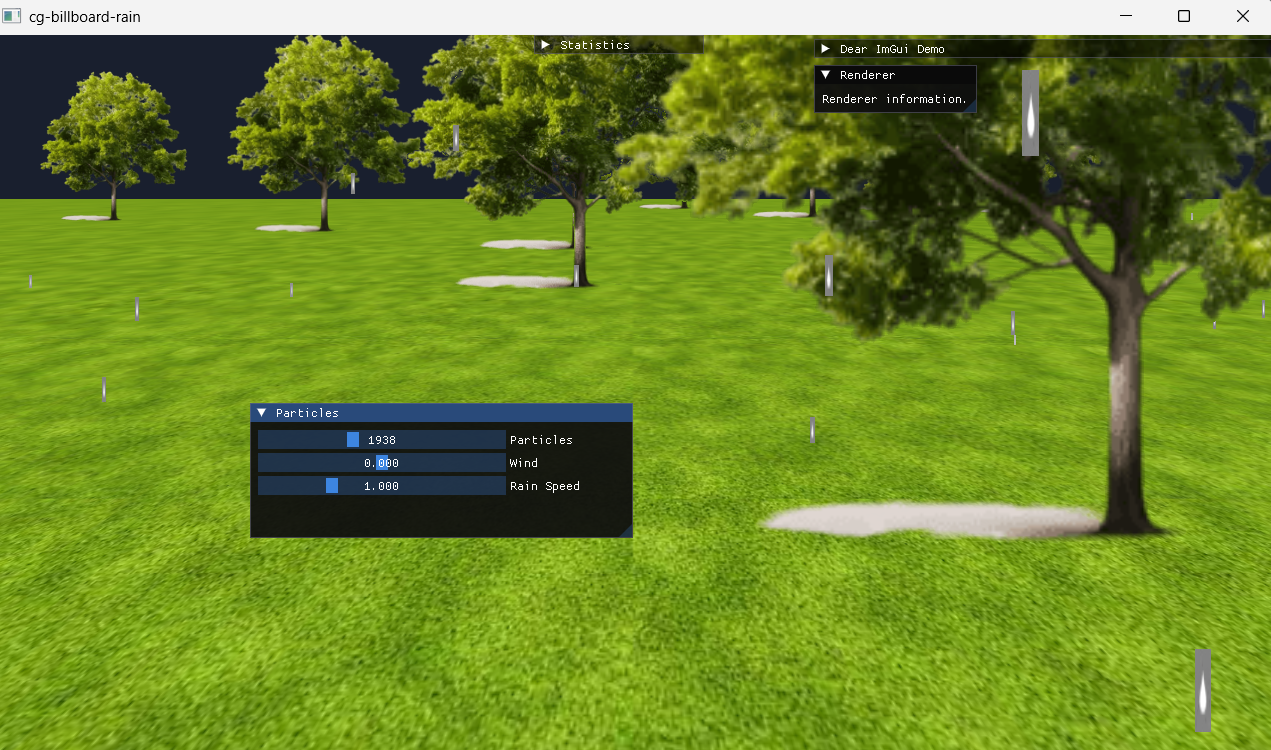
\includegraphics[width=0.9\textwidth]{images/demo.png}
\caption{Resultado general de la simulación.}
\label{fig:escena_general}
\end{figure}

\section{Sistema de partículas}

El sistema de partículas logró representar una lluvia continua utilizando miles de partículas renderizadas simultáneamente.

Cada partícula posee un comportamiento independiente, incluyendo posición, velocidad y reinicio automático al abandonar la zona visible.

Gracias al uso de billboards, todas las partículas permanecen orientadas hacia la cámara, generando una representación visual consistente desde cualquier punto de observación.

La reconstrucción dinámica del sistema permite modificar la cantidad de partículas desde la interfaz gráfica sin necesidad de reiniciar la aplicación.

\section{Sistema de árboles}

Los árboles fueron implementados utilizando billboards de gran tamaño con texturas PNG que incluyen canal alfa.

Cada árbol mantiene siempre su orientación hacia la cámara, simulando modelos tridimensionales con un costo computacional muy reducido.

El algoritmo implementado evita el solapamiento entre árboles mediante una distancia mínima de separación.

Además, cuando un árbol abandona el radio de simulación alrededor del usuario, éste es reposicionado automáticamente delante de la cámara, manteniendo constante la densidad del bosque.

\section{Terreno}

El terreno consiste en un plano texturizado que sigue continuamente la posición horizontal de la cámara.

Este enfoque evita la necesidad de generar un escenario extremadamente grande, reduciendo considerablemente la cantidad de geometría procesada.

Desde la perspectiva del usuario, el terreno aparenta extenderse indefinidamente en todas las direcciones, produciendo una sensación de desplazamiento continuo.

\section{Interfaz gráfica}

La interfaz desarrollada con Dear ImGui permitió modificar diversos parámetros de la simulación durante su ejecución.

Entre los controles disponibles se encuentran:

\begin{itemize}

\item Cantidad de partículas.

\item Intensidad del viento.

\item Velocidad de caída de la lluvia.

\item Información del rendimiento.

\item Posición de la cámara.

\end{itemize}

Las modificaciones realizadas desde la interfaz se reflejan inmediatamente sobre la simulación, permitiendo experimentar distintos escenarios climáticos en tiempo real.

\section{Sistema de audio}

La incorporación de sonido ambiental incrementó significativamente la sensación de inmersión.

El audio de lluvia se reproduce continuamente durante la ejecución del programa.

Su intensidad y velocidad de reproducción cambian automáticamente de acuerdo con la cantidad de partículas presentes en la escena.

De esta manera, una lluvia más intensa produce también una percepción auditiva más fuerte y dinámica.

\section{Sistema meteorológico}

El sistema meteorológico implementado añade relámpagos aleatorios durante la simulación.

Cada relámpago incrementa temporalmente la iluminación del fondo mediante una modificación dinámica del color utilizado por el renderizador.

Posteriormente la intensidad disminuye progresivamente hasta recuperar el estado normal de la escena.

Este efecto visual contribuye a representar una tormenta de manera más realista sin incrementar significativamente el costo computacional.

\section{Evaluación del rendimiento}

Durante las pruebas realizadas se observó un comportamiento estable incluso utilizando varios miles de partículas simultáneamente.

La utilización de billboards para representar tanto la lluvia como los árboles permitió mantener un bajo consumo de memoria y una carga reducida sobre la GPU.

La interfaz gráfica mostró continuamente la cantidad de cuadros por segundo (FPS), permitiendo monitorear el rendimiento de la aplicación mientras se modificaban los parámetros de la simulación.

En equipos con aceleración gráfica compatible con OpenGL 3.3, la simulación mantiene una ejecución fluida para configuraciones de hasta 5000 partículas de lluvia.

\section{Discusión}

Los resultados obtenidos demuestran que es posible construir una simulación visualmente atractiva utilizando técnicas relativamente simples como billboards, sistemas de partículas y renderizado mediante OpenGL.

La arquitectura modular implementada facilitó el desarrollo incremental del proyecto y permitió incorporar nuevas funcionalidades sin modificar significativamente los componentes existentes.

Asimismo, la integración del sistema de audio y los efectos meteorológicos incrementó el nivel de realismo alcanzado por la simulación, ofreciendo una experiencia más inmersiva para el usuario.

\chapter{Conclusiones}

Al finalizar el desarrollo del proyecto se alcanzaron satisfactoriamente los objetivos planteados para la simulación de una tormenta utilizando técnicas de gráficos por computadora basadas en OpenGL.

\begin{enumerate}

\item Se implementó un sistema de partículas capaz de representar lluvia en tiempo real mediante billboards, permitiendo controlar dinámicamente la cantidad de partículas, su velocidad y el efecto del viento.

\item Se desarrolló una arquitectura modular que separa claramente las responsabilidades de renderizado, escena, partículas, audio, interfaz gráfica y efectos meteorológicos, facilitando el mantenimiento y la futura expansión del proyecto.

\item Se implementó un escenario compuesto por un terreno texturizado y árboles representados mediante billboards, optimizando el rendimiento al evitar modelos tridimensionales complejos.

\item Se integró un sistema de audio ambiental utilizando la biblioteca Miniaudio, sincronizando automáticamente el volumen y la velocidad del sonido con la intensidad de la lluvia representada por el sistema de partículas.

\item Se incorporó un sistema meteorológico sencillo basado en relámpagos aleatorios que modifican temporalmente la iluminación general de la escena, incrementando la sensación de realismo sin afectar significativamente el rendimiento.

\item La utilización de Dear ImGui permitió construir una interfaz gráfica intuitiva para modificar en tiempo real los parámetros principales de la simulación y monitorear información de rendimiento como los cuadros por segundo (FPS).

\item Durante las pruebas realizadas, la aplicación mantuvo un comportamiento estable incluso utilizando miles de partículas simultáneamente, demostrando que la utilización de billboards constituye una alternativa eficiente para representar fenómenos naturales como lluvia y vegetación.

\end{enumerate}

En conjunto, el proyecto permitió aplicar diversos conceptos fundamentales de gráficos por computadora, entre ellos transformaciones geométricas, matrices de vista y proyección, texturizado, transparencia mediante canal alfa, renderizado de billboards, sistemas de partículas, integración de audio y organización modular de aplicaciones desarrolladas con OpenGL.

\chapter{Trabajo futuro}

Aunque el proyecto cumple satisfactoriamente con los objetivos propuestos, existen diversas mejoras que podrían incorporarse para incrementar el nivel de realismo y ampliar las funcionalidades de la simulación.

\begin{itemize}

\item Implementar sombras dinámicas generadas por los relámpagos utilizando mapas de sombras (Shadow Mapping).

\item Incorporar efectos de niebla y volumetría para representar condiciones climáticas más realistas durante tormentas intensas.

\item Agregar animaciones de balanceo en los árboles en función de la intensidad y dirección del viento.

\item Implementar múltiples tipos de precipitación, como nieve, granizo o lluvia ligera, reutilizando la arquitectura del sistema de partículas.

\item Incorporar sonidos ambientales adicionales, incluyendo viento, truenos con diferentes intensidades y sonidos producidos por la lluvia al impactar distintas superficies.

\item Desarrollar un sistema de clima dinámico capaz de alternar automáticamente entre cielo despejado, lluvia, tormenta y otros estados meteorológicos.

\item Optimizar el renderizado utilizando técnicas modernas de OpenGL como Instanced Rendering para representar un número considerablemente mayor de partículas y vegetación.

\item Implementar un sistema de terreno basado en alturas (Height Maps) que permita representar montañas, colinas y desniveles en lugar de un plano completamente uniforme.

\item Incorporar modelos tridimensionales para algunos elementos del escenario, combinándolos con billboards para mantener un adecuado equilibrio entre calidad visual y rendimiento.

\item Desarrollar un sistema de iluminación física (PBR) que mejore el comportamiento de los materiales frente a la luz generada por los relámpagos.

\item Añadir soporte para cámaras completamente libres controladas mediante el mouse, permitiendo explorar la escena desde cualquier ángulo.

\item Incorporar un ciclo completo de día y noche con variaciones automáticas de iluminación y condiciones climáticas.

\end{itemize}

La arquitectura modular implementada durante este proyecto facilita la incorporación de estas mejoras, ya que cada componente se encuentra desacoplado del resto del sistema, permitiendo extender la aplicación sin necesidad de modificar significativamente la estructura existente.

\input{chapters/09_repositorio}

\nocite{*}
\bibliographystyle{IEEEtran}

\bibliography{referencias}

\end{document}